%%
%% This is file `main.tex' based on `sample-sigconf.tex' (q.v. for spurce of that,
%%
%% IMPORTANT NOTICE:
%% 
%% For the copyright see the original source file `sample-sigconf.tex'
%% in the `Sample' folder.
%%
%% For distribution of the original source see the terms
%% for copying and modification in the file samples.dtx.
%% 
%% This generated file may be distributed as long as the
%% original source files, as listed above, are part of the
%% same distribution. (The sources need not necessarily be
%% in the same archive or directory.)
%%
%% Commands for TeXCount
%TC:macro \cite [option:text,text]
%TC:macro \citep [option:text,text]
%TC:macro \citet [option:text,text]
%TC:envir table 0 1
%TC:envir table* 0 1
%TC:envir tabular [ignore] word
%TC:envir displaymath 0 word
%TC:envir math 0 word
%TC:envir comment 0 0
%%
%%
%% The first command in your LaTeX source must be the \documentclass command.

%% NOTE that a single column version is required for 
%% submission and peer review. This can be done by changing
%% the \doucmentclass[...]{acmart} in this template to 
%%\documentclass[manuscript,review,anonymous]{acmart}
%% This version is used for drafting and final submission
\documentclass[sigconf]{acmart}
\usepackage{float}


%% 
%% To ensure 100% compatibility, please check the white list of
%% approved LaTeX packages to be used with the Master Article Template at
%% https://www.acm.org/publications/taps/whitelist-of-latex-packages 
%% before creating your document. The white list page provides 
%% information on how to submit additional LaTeX packages for 
%% review and adoption.
%% Fonts used in the template cannot be substituted; margin 
%% adjustments are not allowed.

%%
%% \BibTeX command to typeset BibTeX logo in the docs
\AtBeginDocument{%
  \providecommand\BibTeX{{%
    \normalfont B\kern-0.5em{\scshape i\kern-0.25em b}\kern-0.8em\TeX}}}

%% Rights management information.  This information is sent to you
%% when you complete the rights form.  These commands have SAMPLE
%% values in them; it is your responsibility as an author to replace
%% the commands and values with those provided to you when you
%% complete the rights form.
\setcopyright{acmlicensed}
\copyrightyear{2024}
\acmYear{2024}

%% These commands are for a PROCEEDINGS abstract or paper.
%
%  Uncomment \acmBooktitle if th title of the proceedings is different
%  from ``Proceedings of ...''!
%
%\acmBooktitle{Woodstock '18: ACM Symposium on Neural Gaze Detection,
%  June 03--05, 2018, Woodstock, NY} 
\acmISBN{978-1-4503-XXXX-X/18/06}


%%
%% Submission ID.
%% Use this when submitting an article to a sponsored event. You'll
%% receive a unique submission ID from the organizers
%% of the event, and this ID should be used as the parameter to this command.
%%\acmSubmissionID{123-A56-BU3}

%%
%% For managing citations, it is recommended to use bibliography
%% files in BibTeX format.
%%
%% You can then either use BibTeX with the ACM-Reference-Format style,
%% or BibLaTeX with the acmnumeric or acmauthoryear sytles, that include
%% support for advanced citation of software artefact from the
%% biblatex-software package, also separately available on CTAN.
%%
%% Look at the sample-*-biblatex.tex files for templates showcasing
%% the biblatex styles.
%%

%%
%% The majority of ACM publications use numbered citations and
%% references.  The command \citestyle{authoryear} switches to the
%% "author year" style.
%%
%% If you are preparing content for an event
%% sponsored by ACM SIGGRAPH, you must use the "author year" style of
%% citations and references.
%% Uncommenting
%% the next command will enable that style.
%%\citestyle{acmauthoryear}

%%
%% end of the preamble, start of the body of the document source.

%% % Location of your graphics files for figures, here a sub-folder to the main project folder
\graphicspath{{./images/}} 


\begin{document}

%%
%% The "title" command has an optional parameter,
%% allowing the author to define a "short title" to be used in page headers.
\title{Competitive Esports Network: A Relational Approach to
Tournament Management \\ Phase III}

%%
%% The "author" command and its associated commands are used to define
%% the authors and their affiliations.
%% Of note is the shared affiliation of the first two authors, and the
%% "authornote" and "authornotemark" commands
%% used to denote shared contribution to the research.
\author{Wyatt Fischer}
\email{fisc7842@vandals.uidaho.edu}
\affiliation{
    \institution{University of Idaho}
    \city{Moscow}
    \state{Idaho}
    \country{USA}
}

\author{Nastia Kossiak}
\email{koss0519@vandals.uidaho.edu}
\affiliation{
    \institution{University of Idaho}
    \city{Moscow}
    \state{Idaho}
    \country{USA}
}
\author{Brandon Lunney}
\email{lunn2076@vandals.uidaho.edu}
\affiliation{
    \institution{University of Idaho}
    \city{Moscow}
    \state{Idaho}
    \conutry{USA}
}

%%
%% By default, the full list of authors will be used in the page
%% headers. Often, this list is too long, and will overlap
%% other information printed in the page headers. This command allows
%% the author to define a more concise list
%% of authors' names for this purpose.
\renewcommand{\shortauthors}{Fischer, Kossiak, and Lunney}

%%
%% The abstract is a short summary of the work to be presented in the
%% article.
\begin{abstract}
  An update on the E-Sports Competitive Network is presented. A tool that is designed to showcase e-sports players, teams, and tournaments through a graphic interface while utilizing a relational database. The description of the current working prototype is given as well as changes to the entity relational model and tech stack since the previous report. Showcases of all current web pages of the project are detailed with mass database population and manual insertion. Implementation details of the three key queries utilized by the tool are described. Lastly, a reflection on the timeline since project start.
\end{abstract}

%%
%% The code below is generated by the tool at: http://dl.acm.org/ccs.cfm
%% Please copy and paste the code instead of the example below.
%%
\begin{CCSXML}
<ccs2012>
 <concept>
  <concept_id>00000000.0000000.0000000</concept_id>
  <concept_desc>Information Systems</concept_desc>
  <concept_significance>500</concept_significance>
 </concept>
 <concept>
  <concept_id>00000000.00000000.00000000</concept_id>
  <concept_desc>Applied Computing</concept_desc>
  <concept_significance>300</concept_significance>
 </concept>
</ccs2012>
\end{CCSXML}

\ccsdesc[500]{Relational Databases}
\ccsdesc[300]{Computer Games}

%%
%% Keywords. The author(s) should pick words that accurately describe
%% the work being presented. Separate the keywords with commas.
\keywords{Esports, Relational Databases, MySQL, Cytoscape, Network Visualization, Python}

%%
%% This command processes the author and affiliation and title
%% information and builds the first part of the formatted document.
\maketitle

\section{Introduction}
E-Sports is one of the fastest growing media in recent years. The biggest e-sports events can even receive upwards of 5.5 million views. With a wide range of games, including titles such as \textit{League of Legends}, \textit{Counter-Strike}, and \textit{Dota 2}, the industry has developed a vast ecosystem of professional teams and large-scale tournaments. However, unlike it's real life counterpart e-sports does not have near the amount of statistical analysis tools as regular sports. These tools allow coaches, fans, and researchers to better understand performance trends, strategic strengths, and the relationships between teams across seasons. This was the motivation behind the \textit{E-Sports Competitive Network}. For this project we will be implementing a relational database to facilitate statistical analysis of e-sports players and teams across several seasons and games. We will then utilizing that database to visually communicate the information in a graph format.\\
The requirements of this project are we facilitate multiple types of nodes, in this instance this is players, teams, and the tournaments themselves. This project will also allow for several edges types, such that teammates, played in, and played for. We also allow for multi-graph support, specifically the ability for a node to belong to several graphs and by extension edges to multiple graphs as well. There will also feature a minimum set of queries available, such as an h-index filter or for our purposes a win rate filter for the teams and players. As well as a Co-Author network which for this system will be a teammate network.  Lastly, there will be a Q1 journal influence network. However, for our purposes this will be a Q1 tournament influence network, where the Q1-Q4 will be determined based on which quartile the prize pool falls into. Then we will find all teams and by extension the players that participated in that tournament.
\section{Prototype Description}
The E-Sports Competitive Network prototype is designed to address the lack of advanced statistical analysis tools in competitive gaming. This prototype introduces a relational database system that models graph connections between players, teams, and tournaments across multiple games. The prototype implements three key analytical queries. First, a teammate influence network that constructs a teammate graph showing how players are connected. Second, an h-index filer, identifies consistently high-performing teams based on either participation or number of wins. Lastly, a Q1-Journal Influence Network that identifies the most impactful tournaments based on prize pool and connects them to the participating teams. The prototype also allows for database population with a custom web scrapping tool as well as several web pages to manually insert information. 
\section{Updated Entity Relation Model}
In previous reports Figure 1 depicts the entity relation diagram. Which featured several tables for players, teams, tournaments and the relationships between them, played-for, played-in. This worked for the initial prototype allowing for the basic create, read, update, and delete operations within the database. However, as we began to implement the graph presentation with Cytoscape we faced issues implementing the multi-graph support without implementing complex queries. This lead to a refinement to Figure 2 which showcases the updated entity relation model.
\begin{figure}[H]
    \centering
    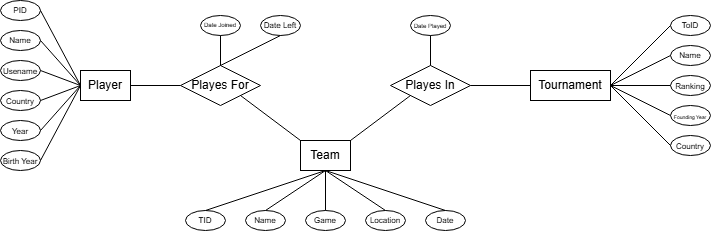
\includegraphics[width=1\linewidth]{images/ERDiagram.png}
    \caption{Old Entity Relation Diagram}
    \label{fig:placeholder}
\end{figure}

The benefits of this model is rather than having three different types of entities for each team, player, and tournament we simply have a Node entity. Each Node has a NodeID which acts as the primary key. Then the team, player, or tournament attribute is stored withing the NodeType value. Since each team, player, and tournament has different amount of attributes stored with it the Attributes column is a JSON file allowing for flexible metadata on the node. \\
Similarly, rather than having two different tables for the played-for and played-in relationship we consolidated it to one Edge entity. Each edge has a an EdgeID acting as the primary key. As well as two node id's, SourceNodeID and TargetNodeID, which describe the nodes the edge connects as well as are foreign keys to the node table. For the same reasons as the node entity we gave the edge entity and EdgeType value which holds the played-in or played-for relationship. Lastly, since each relasonship holds a different number of descriptors edges have a MetaData value which acts identically to the Attributes column of nodes.\\
To facilitate the multi-graph support we've added a new entity to represent the graphs themselves. Each graph has a GraphID which is the primary key of the table. Each graph also has a name that can be displayed. In addition, each graph has a description to further add details to the graph.
We've also added a new relationship between the entities, Member of, this represents the relationship between a graph and a node or edge. Each membership has it's own MemeberID which acts as the primary key. A nodeID or edgeID which determines which entity belongs to the graph. The graphID to determine which graph the entity belongs to. This schema allows for easy graph integration and multi-graph support, in addition for further expansion if we decide to add more types of nodes or edges.
\begin{figure}[H]
    \centering
    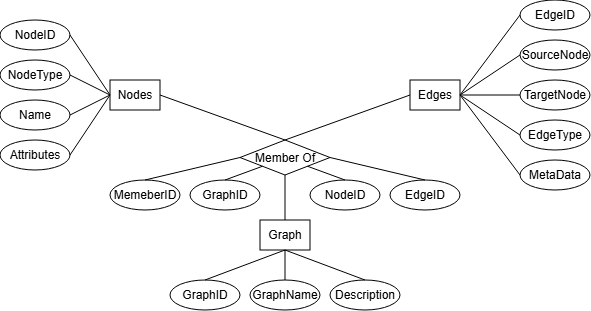
\includegraphics[width=1\linewidth]{images/UpdatedERDiagram.png}
    \caption{Updated Entity Relation Model}
    \label{fig:placeholder}
\end{figure}
\section{Tech Stack}
Likewise to past reports this project utilizes three different categories of technology. A database, back-end processing, and front-end/presentation.

\subsection{Database}
In previous reports the database we decided on was \textbf{MySQL}, which is based around the client-server model. To simplify development and improve collaboration we've transitioned to \textbf{SQLite}, a lightweight relational database that follows a serverless architecture. This design makes it extremely easy to set up and allows team members to share the database simply by distributing the file.
\subsection{Back-End}
For the back end we've utilized \textbf{Python} for it's expansive libraries and data analysis tools. We leveraged Python’s frameworks and libraries to handle core logic and data interaction with the SQLite database. Discussed later, we utilized Flask for webpage routing and Playwright to populate the database.
\subsection{Front-End}
The front end utilizes HTML and CSS for the webpage templates as well as the presentation. To present the graph presentation of the network we utilize Cytoscape which is an open-source network visualizer. Which allows us to render complex relationships in an intuitive way. Through its JavaScript integration we are able to embed interactive graphs directly into the webpage.

\section{Implementation}
\subsection{Populating the Database}
To populate the initial database we've developed a web scrapper that utilizes Playwright to load web pages and scrape the information from the html tags then inserts them into the database. The scraper checks for duplicate nodes, in that case the node's attributes are updated. In addition, the scrapper creates the respective edges as well. Below is a list of webpages where we scrape the information.

\begin{enumerate}
    \item https://prosettings.net/players/
    \item https://en.wikipedia.org/wiki/
    \item https://liquipedia.net/valorant/S-Tier\_Tournaments
    \item https://liquipedia.net/valorant/A-Tier\_Tournaments
\end{enumerate}
In addition to the web scraper, the project also includes several dedicated webpages that allow users to insert data directly into the database. These pages utilize forms to fill in a SQL statement that is then executed by the database manager. Figures 3 showcases the database insertion webpages.
\begin{figure}[H]
    \centering
    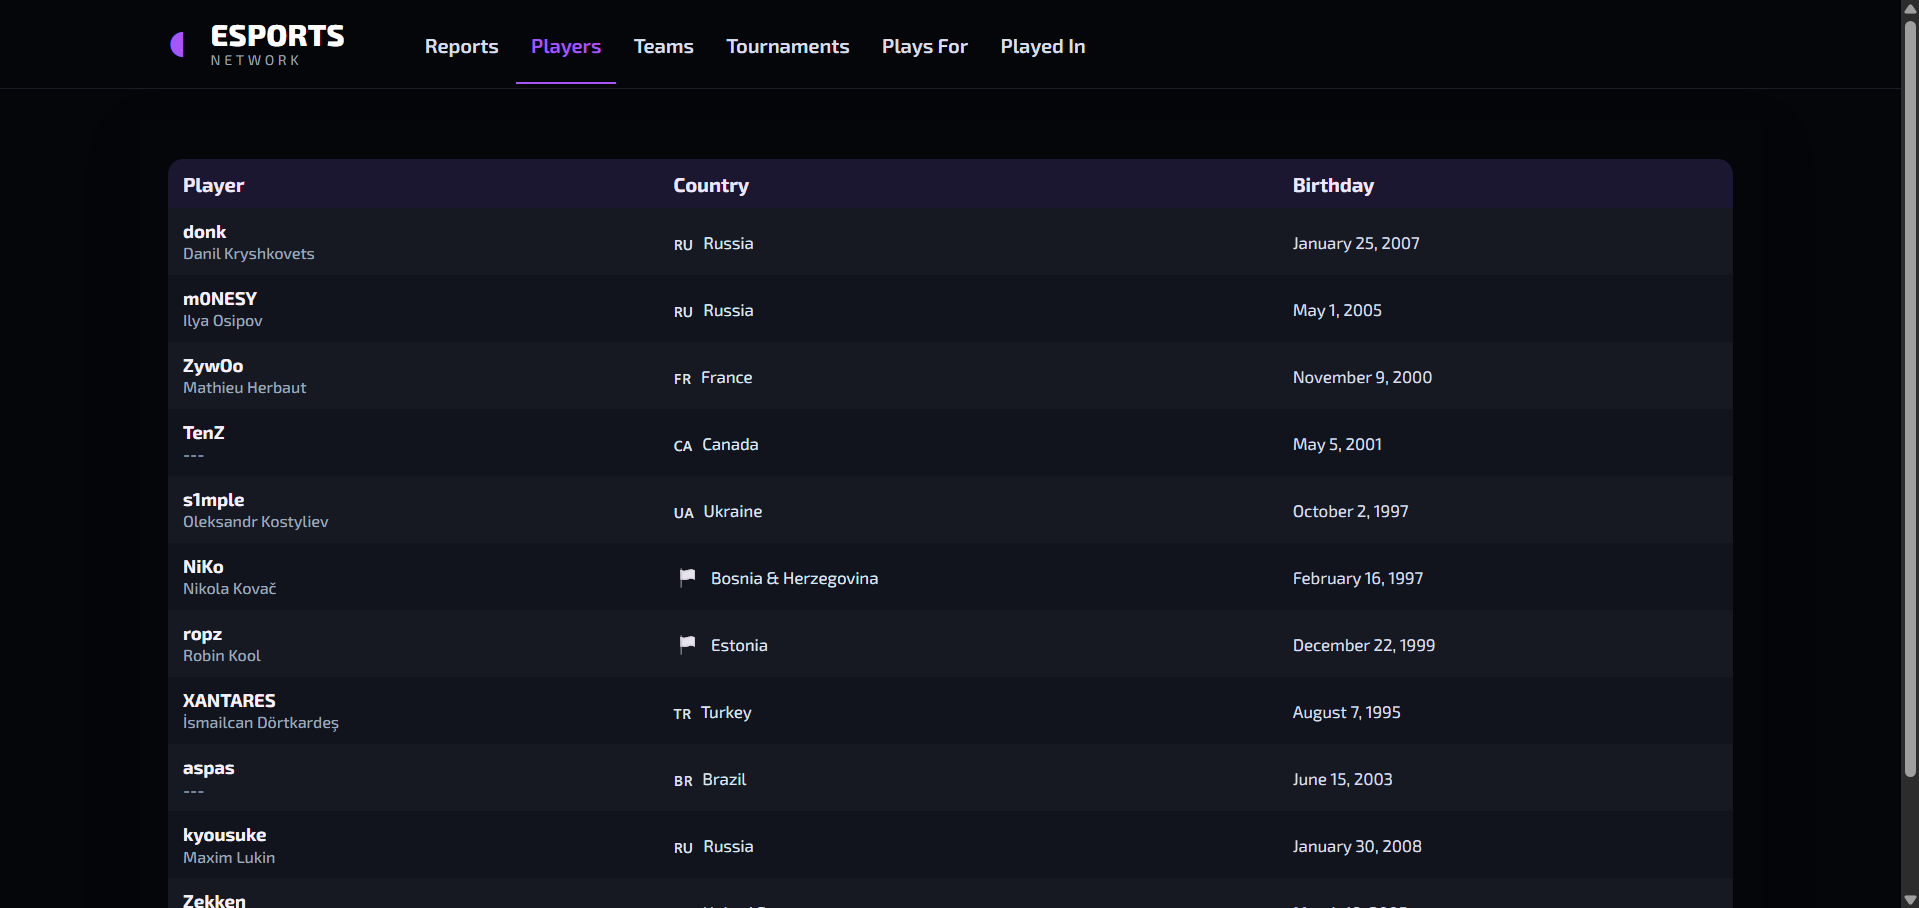
\includegraphics[width=1\linewidth]{images/ESports-Players.png}
    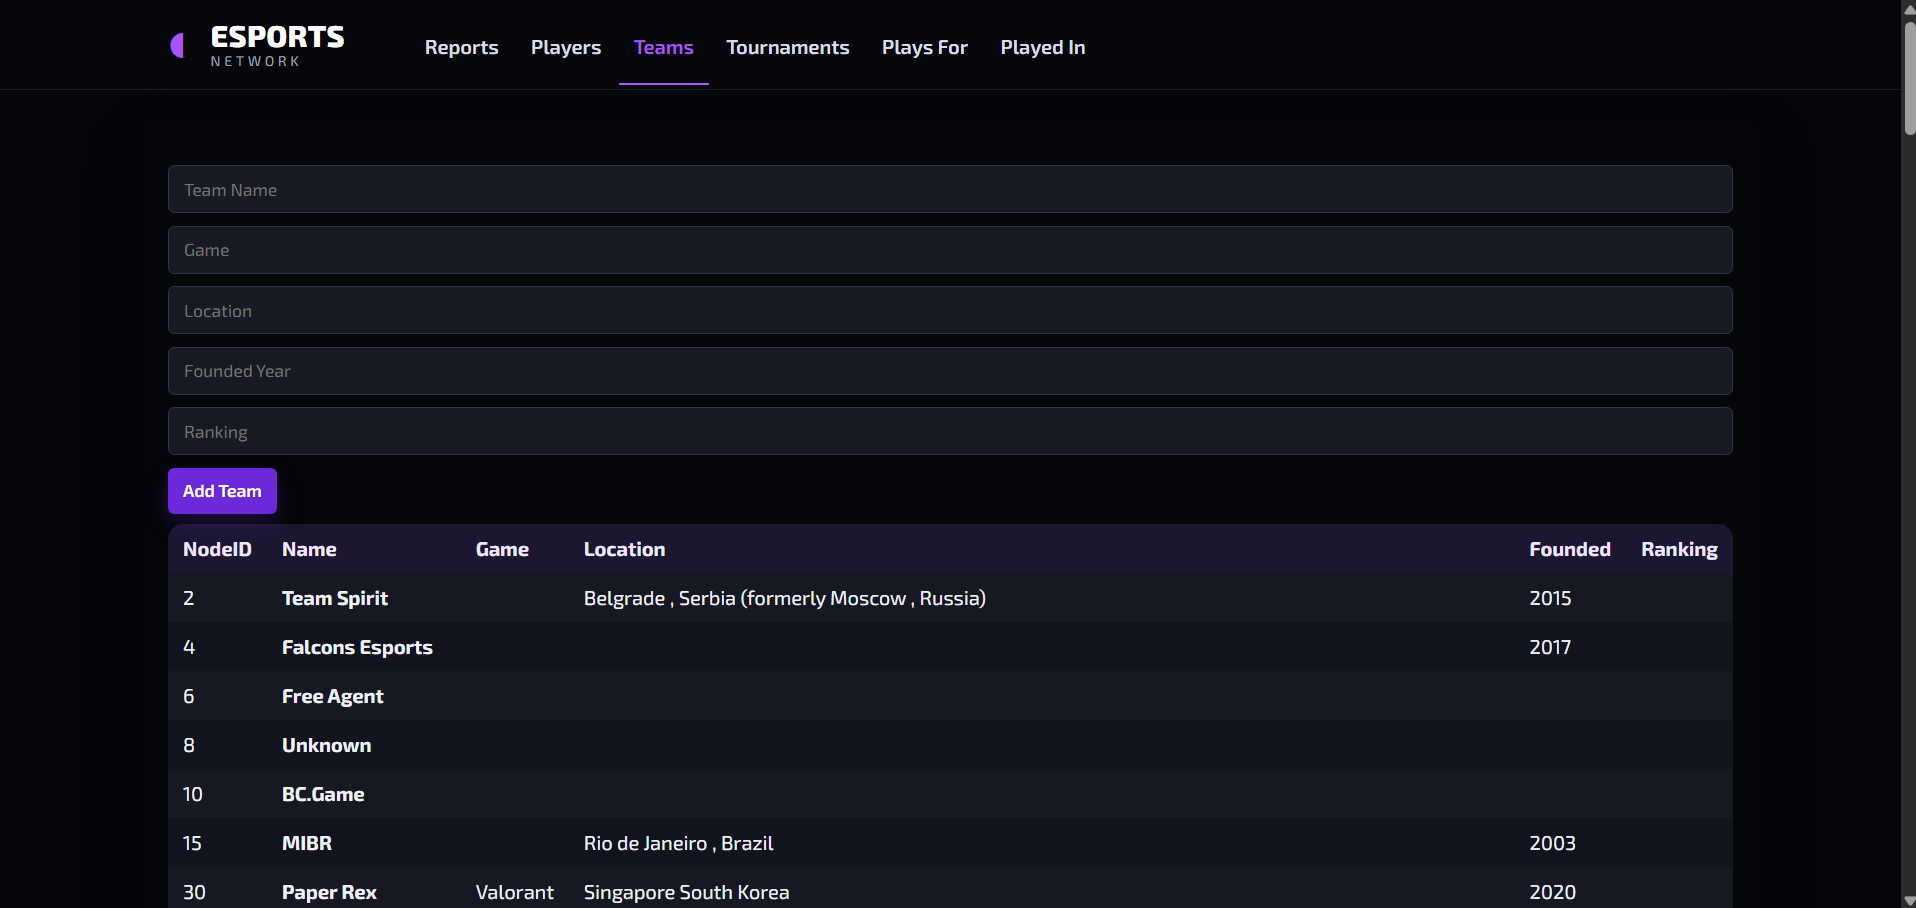
\includegraphics[width=1\linewidth]{images/ESports-Teams.png}
    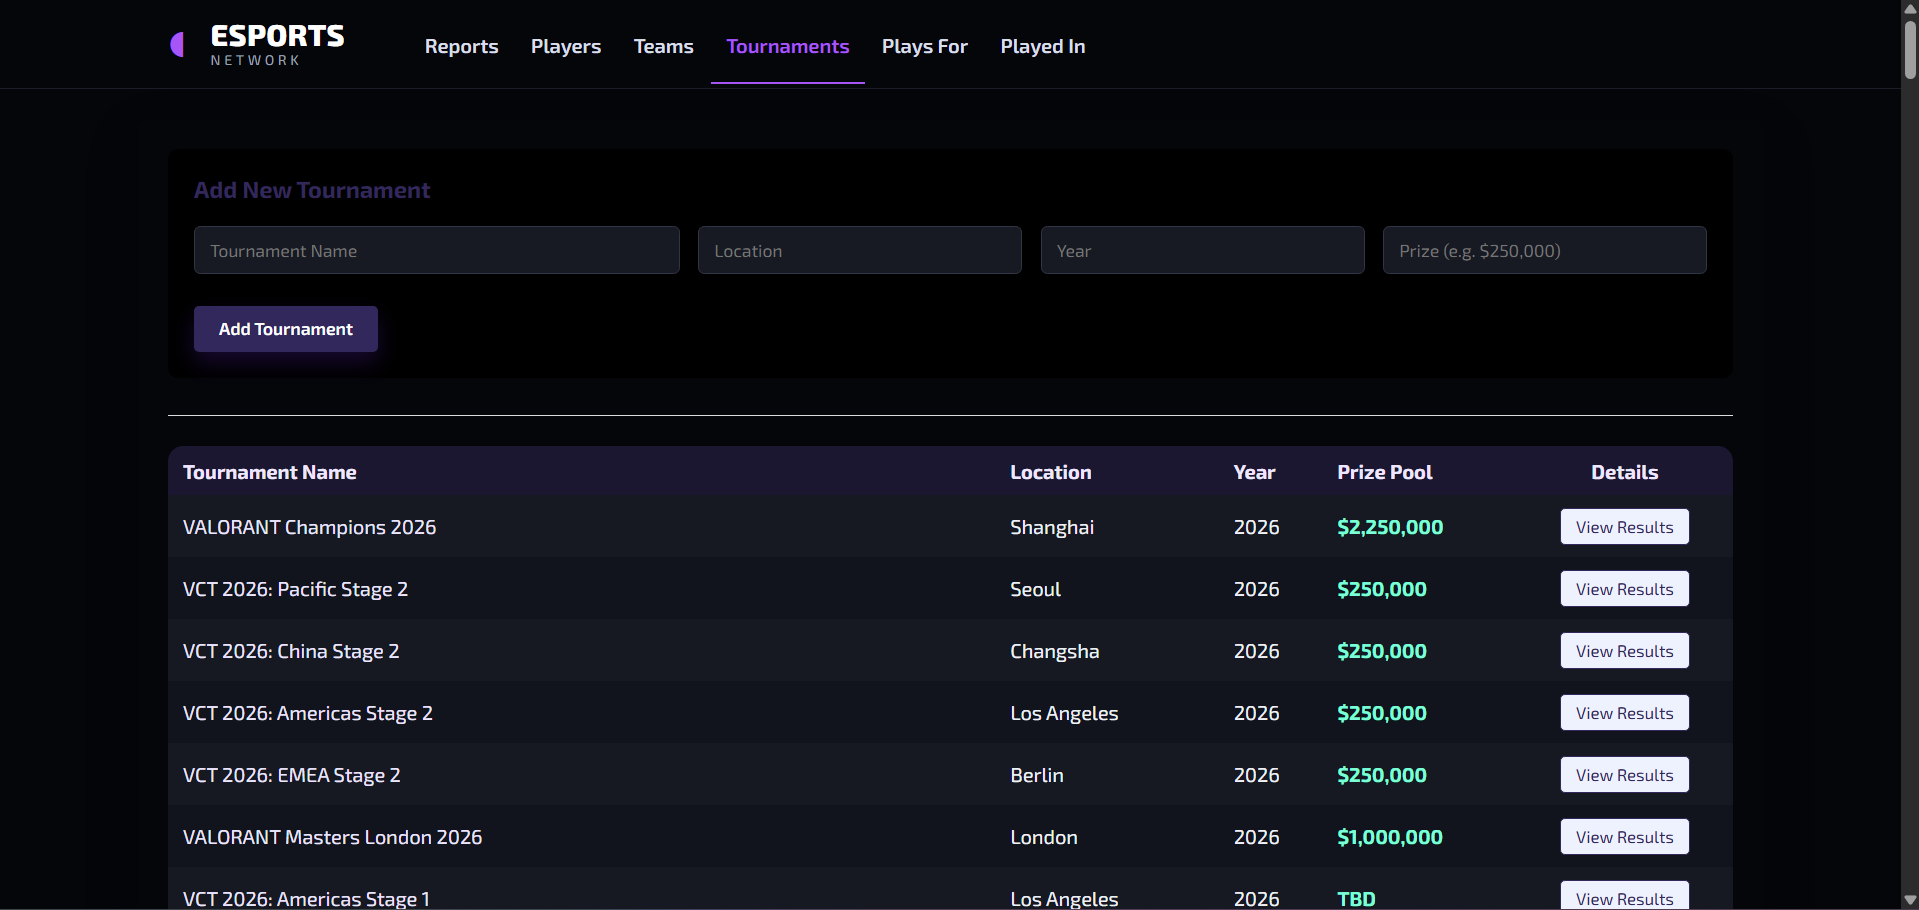
\includegraphics[width=1\linewidth]{images/ESports-Tournaments.png}
    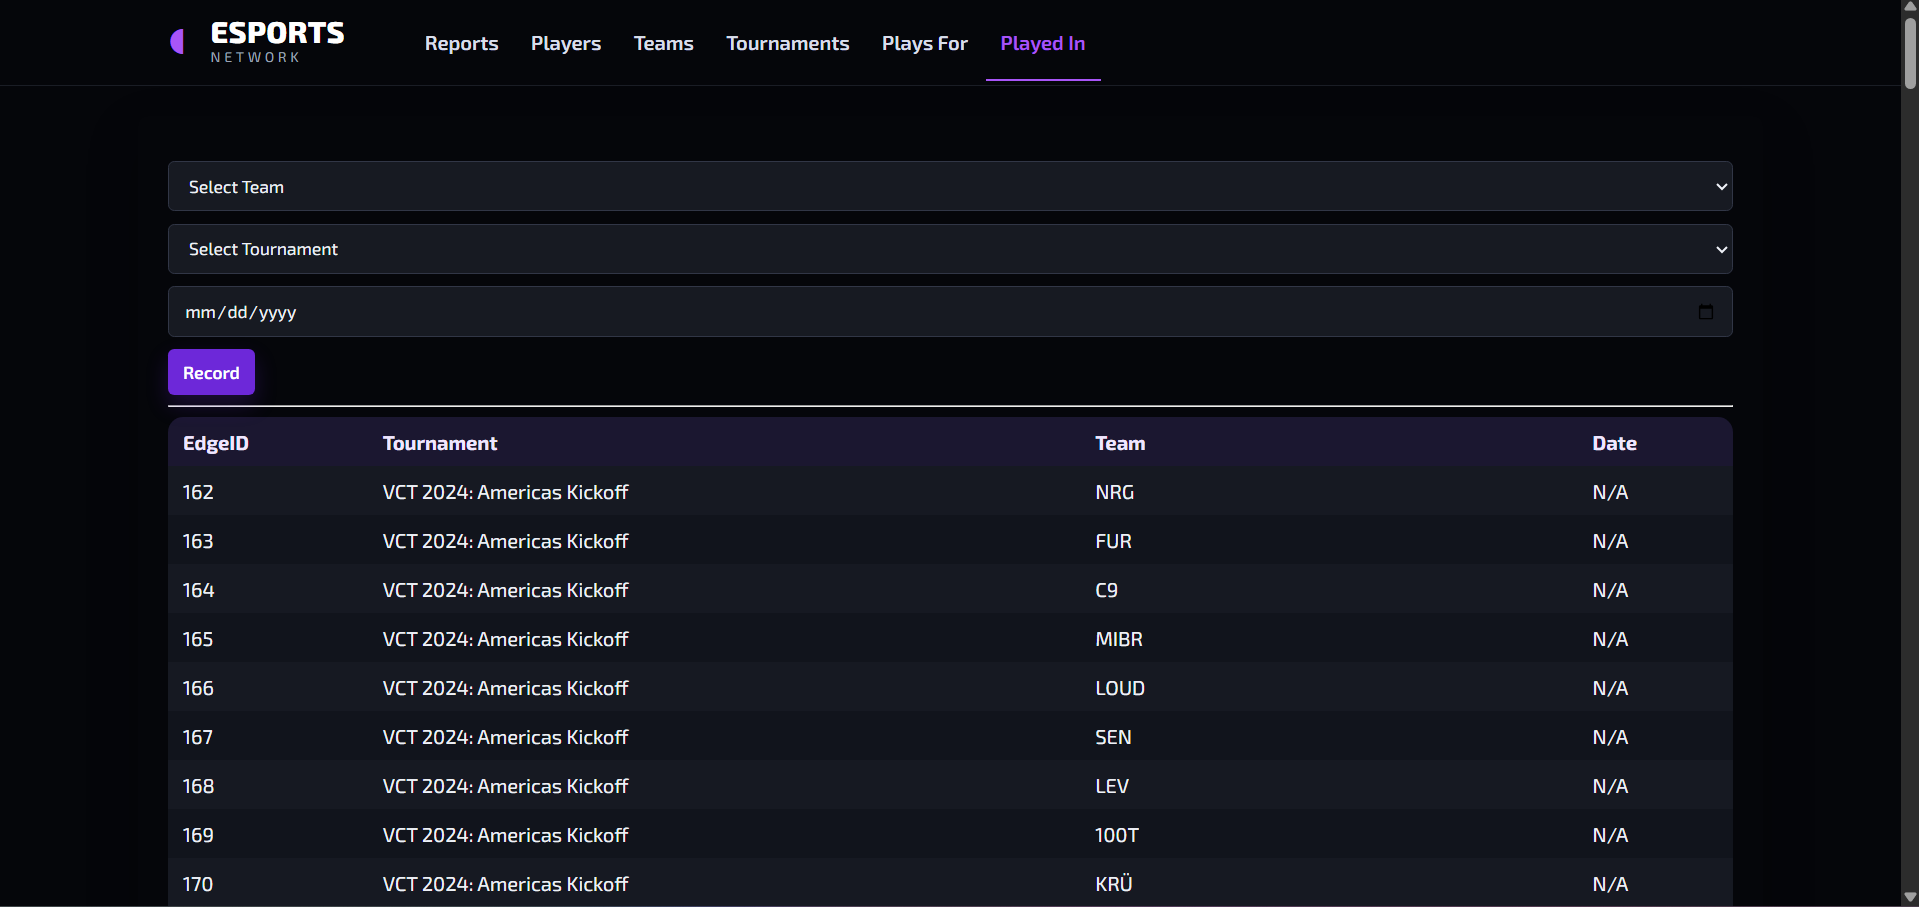
\includegraphics[width=1\linewidth]{images/ESports-PlayedIn.png}
    \label{fig:placeholder}
\end{figure}
\begin{figure}[H]
    \centering
    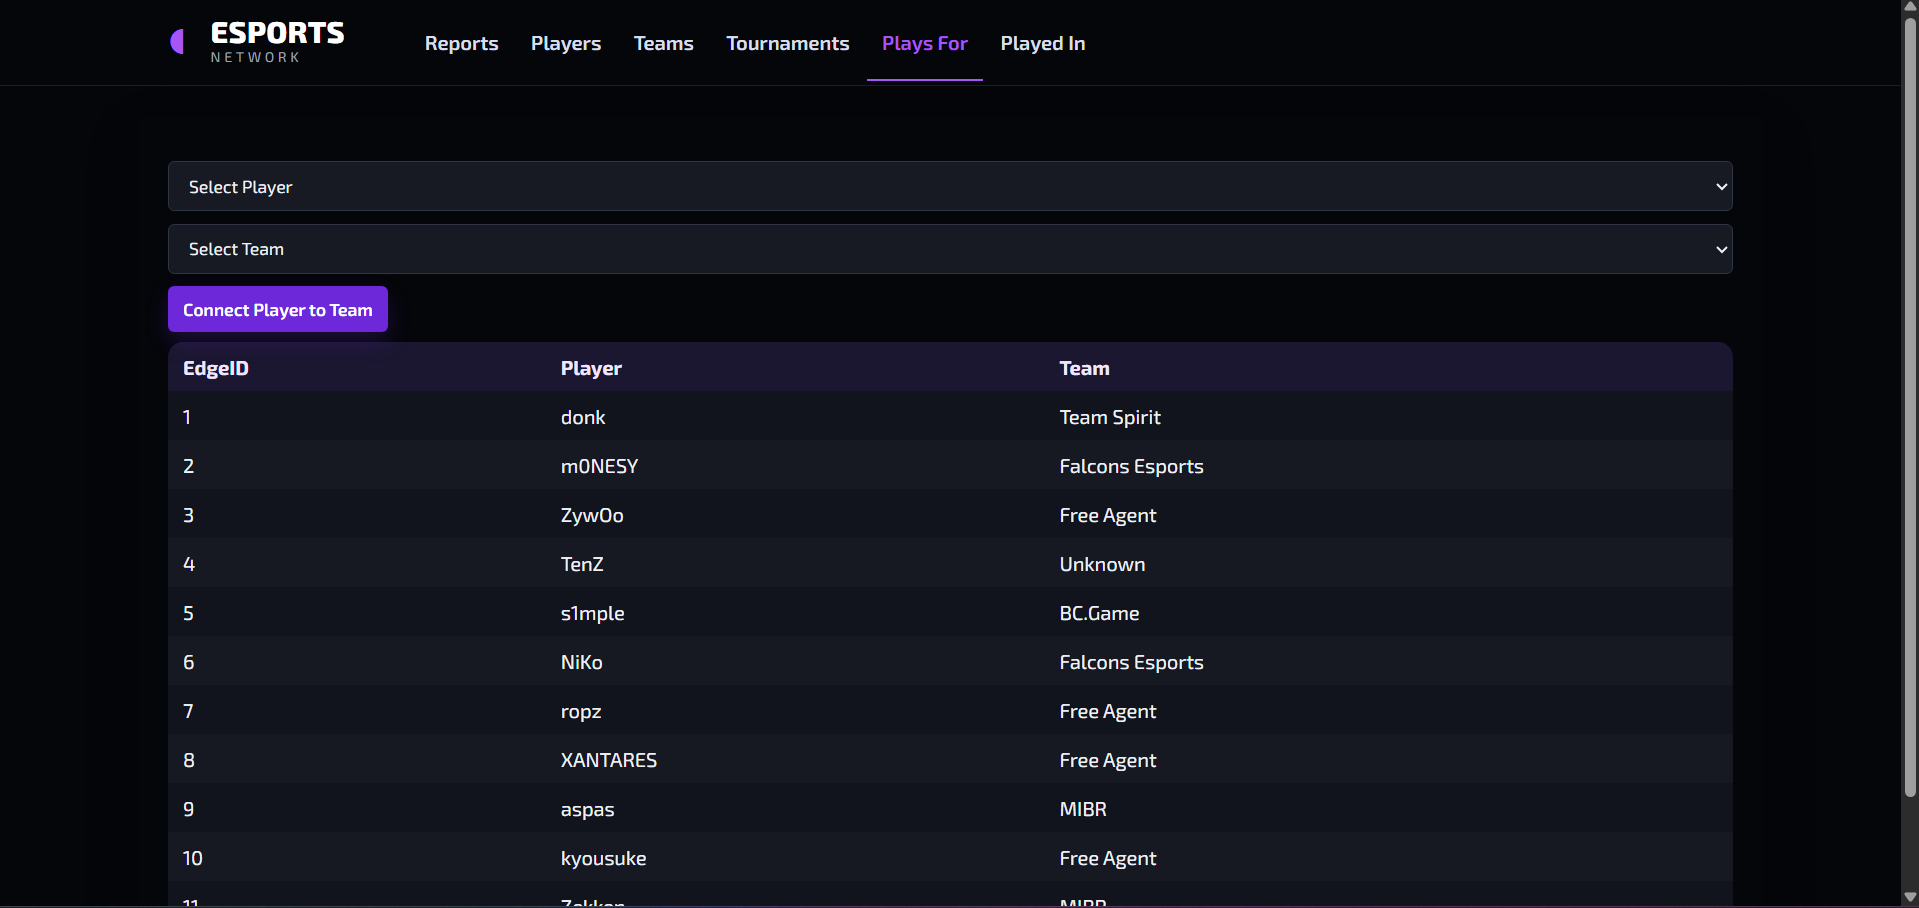
\includegraphics[width=1\linewidth]{images/ESports-PlaysFor.png}
    \caption{Database Insertion Webpages}
    \label{fig:placeholder}
\end{figure}

\subsection{Reports Page}
As mentioned previously the project utilizes Flask to handle webpage routing. Each webpage calls from the database and then fills in the template html page with the returned information from the database. The front page get the entire database then utilizes Cytoscape's java script integration to present the information. Figure 4 showcases the front webpage.
\begin{figure}[H]
    \centering
    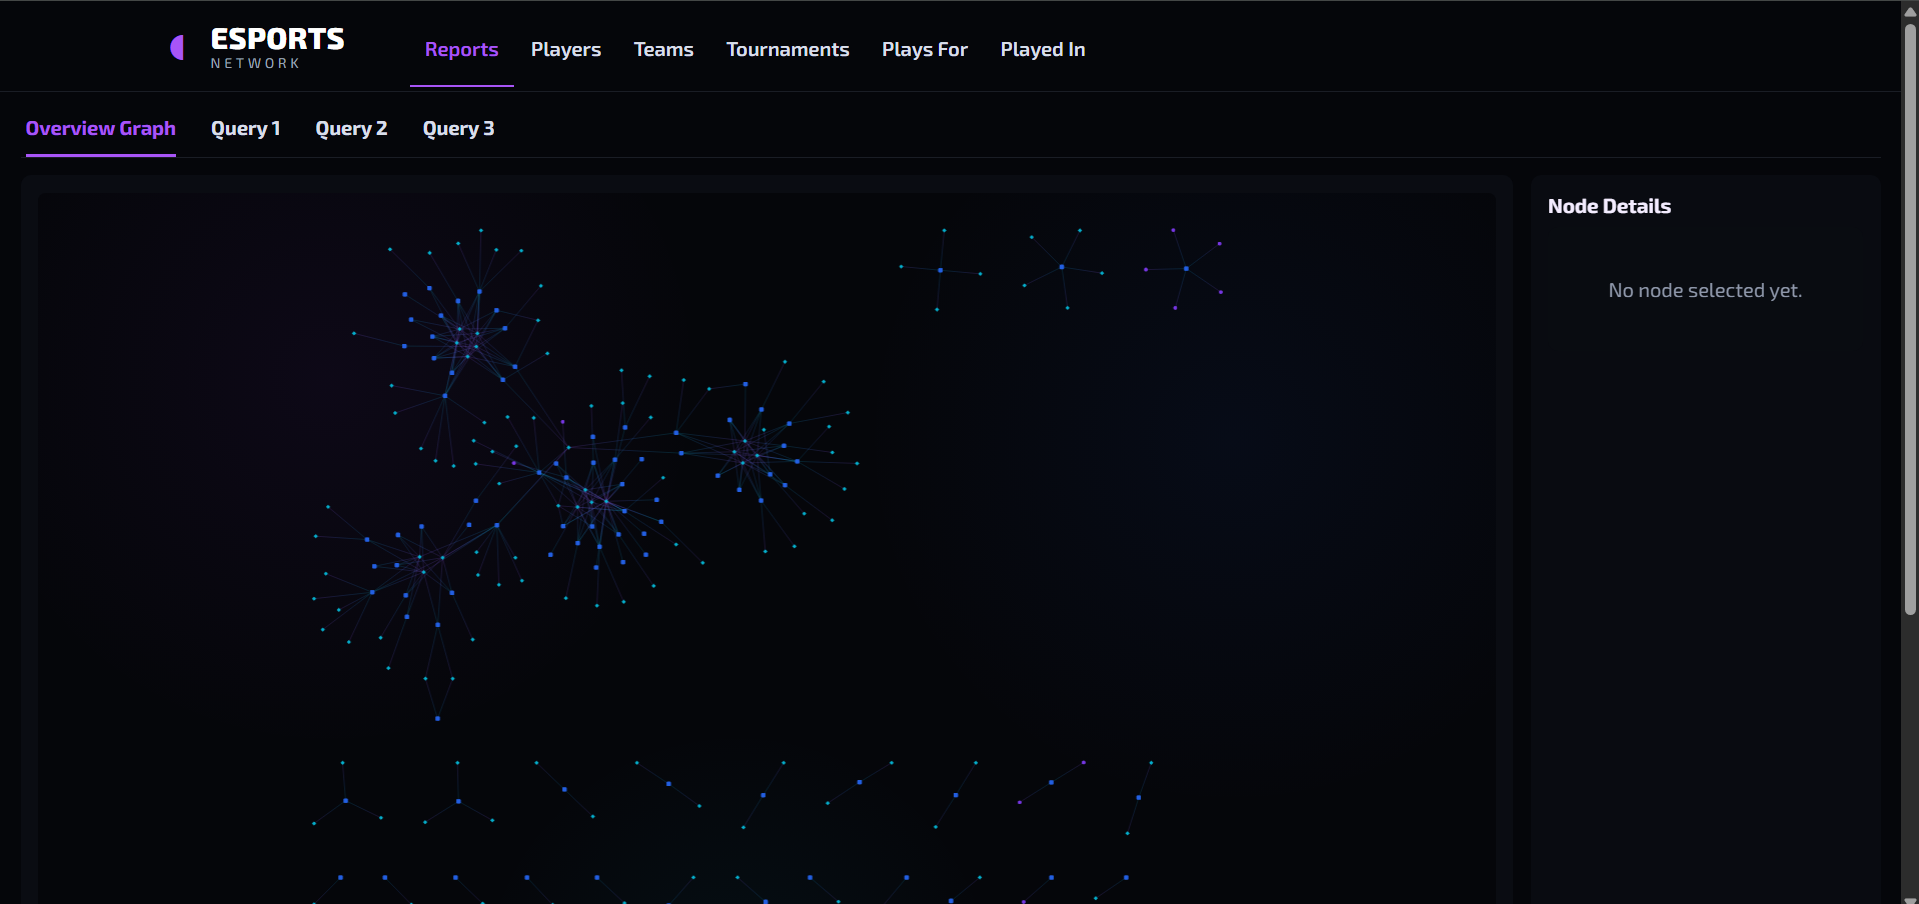
\includegraphics[width=1\linewidth]{images/ESports-Reports.png}
    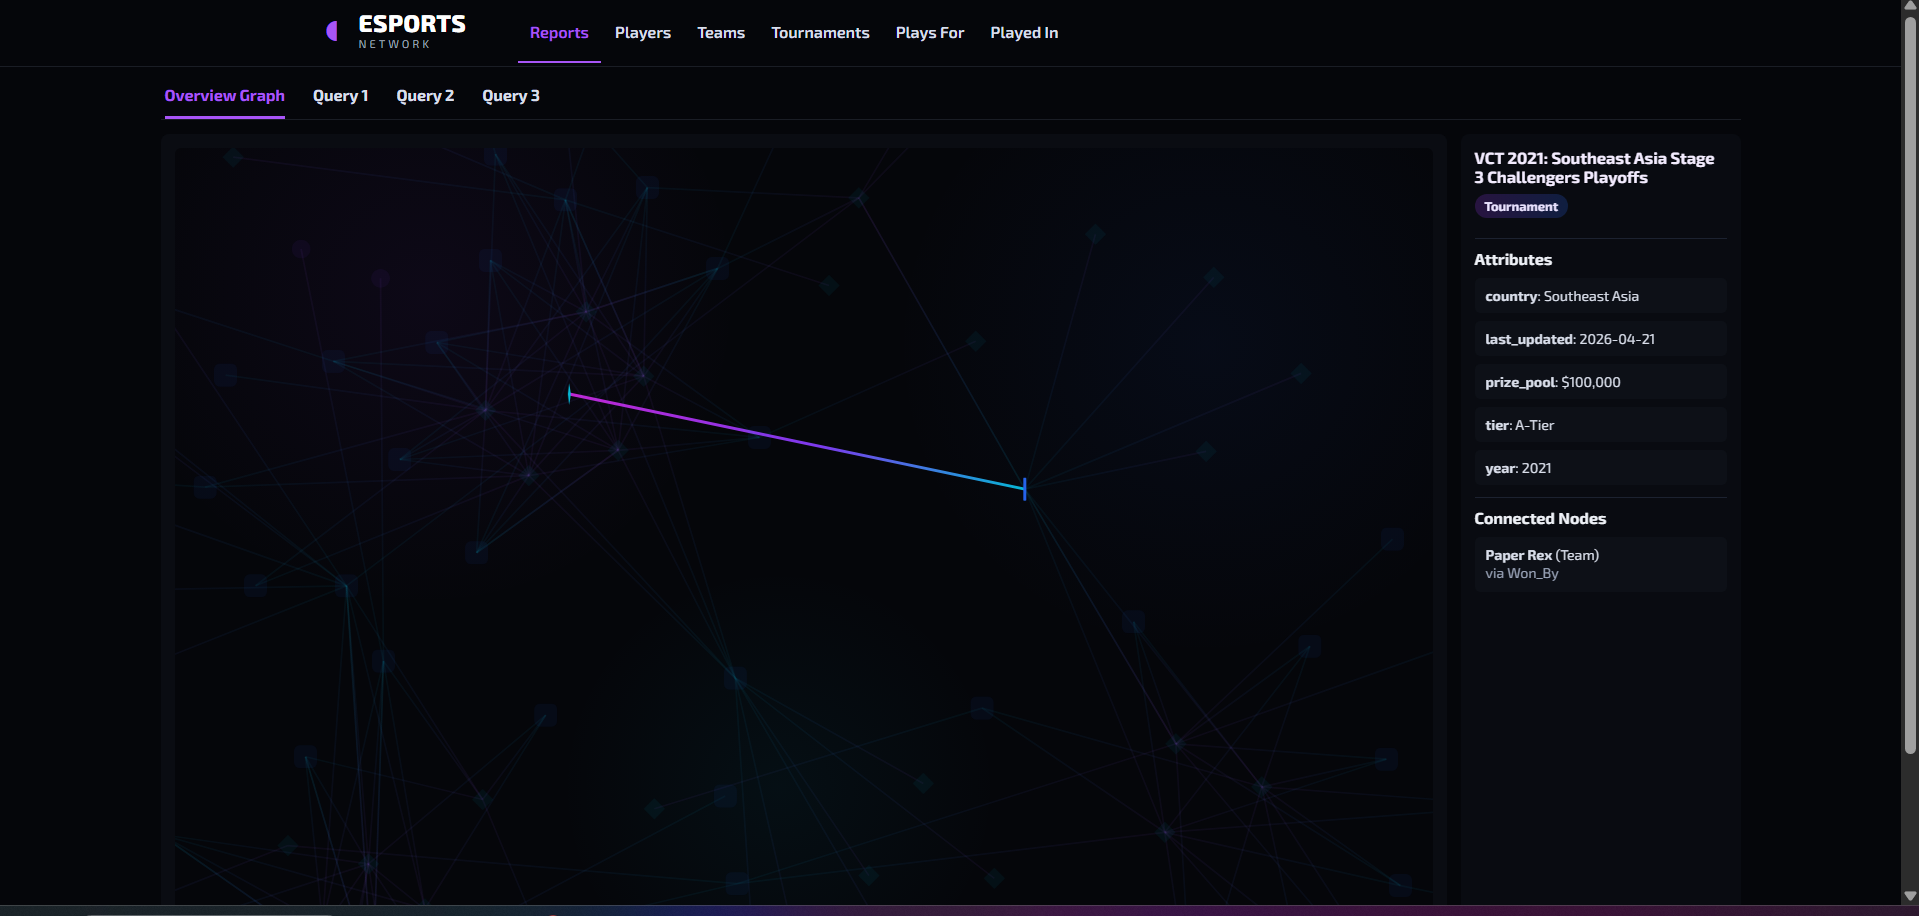
\includegraphics[width=1\linewidth]{images/ESports-ReportsExample.png}
    \caption{Reports Web Page}
    \label{fig:placeholder}
\end{figure}

\subsection{Query 1}
For this project the initial guidelines were to implement a \textit{Co-Author Network}. For this specific project we implemented a \textit{Teammate Network} which takes in a specific player and then returns all other players that play for the same team as that player. The webpage executed the below queries to get the respective nodes and edges.
Which selects all nodes that are connected to the same team as the given player then gets all appropriate edges. Figure 5 also showcases the webpage itself.

\begin{verbatim}
SELECT DISTINCT n.NodeID, n.Name, n.NodeType, n.Attributes
    FROM Nodes n
    JOIN GraphMemberships gm ON gm.NodeID = n.NodeID
    WHERE gm.GraphID = 1
    AND n.NodeType IN ("Player", "Team")
    ORDER BY n.NodeType, n.Name
SELECT DISTINCT e.EdgeID, e.SourceNodeID, e.TargetNodeID, 
e.EdgeType, e.Metadata
    FROM Edges e
    JOIN GraphMemberships gm ON gm.EdgeID = e.EdgeID
    WHERE gm.GraphID = 1
    AND e.EdgeType = "Plays_For"
\end{verbatim}

\begin{figure}[H]
    \centering
    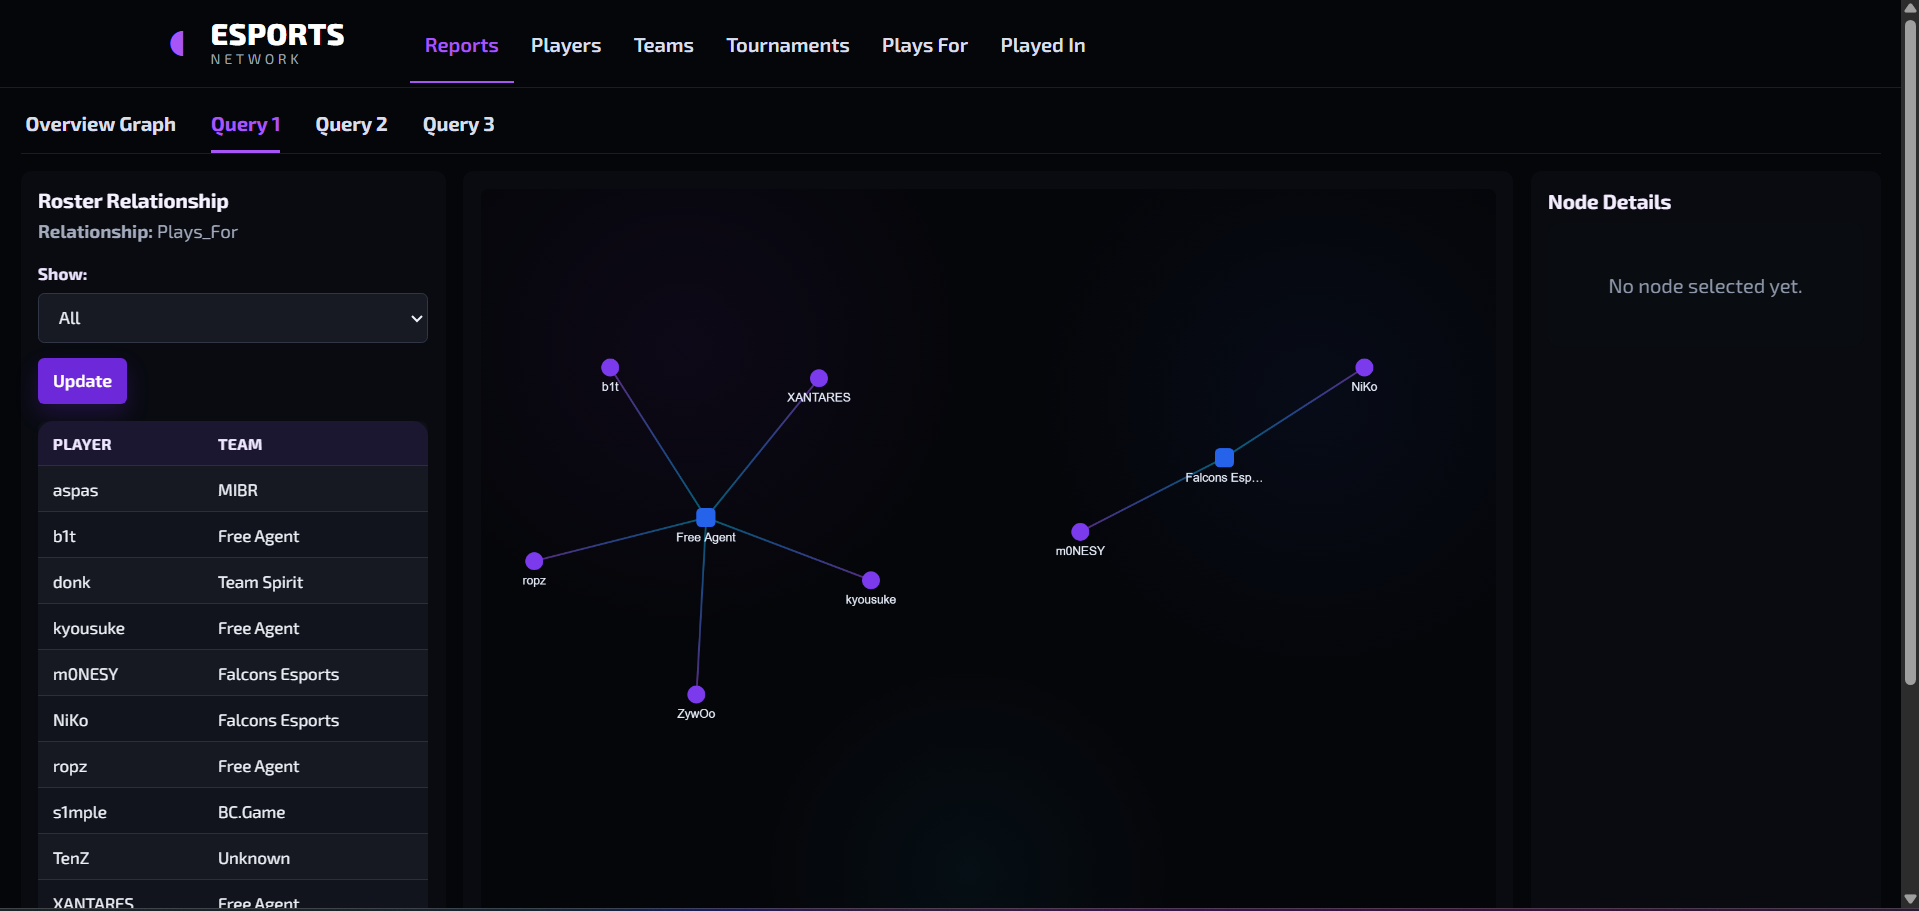
\includegraphics[width=1\linewidth]{images/ESports-Q1.png}
    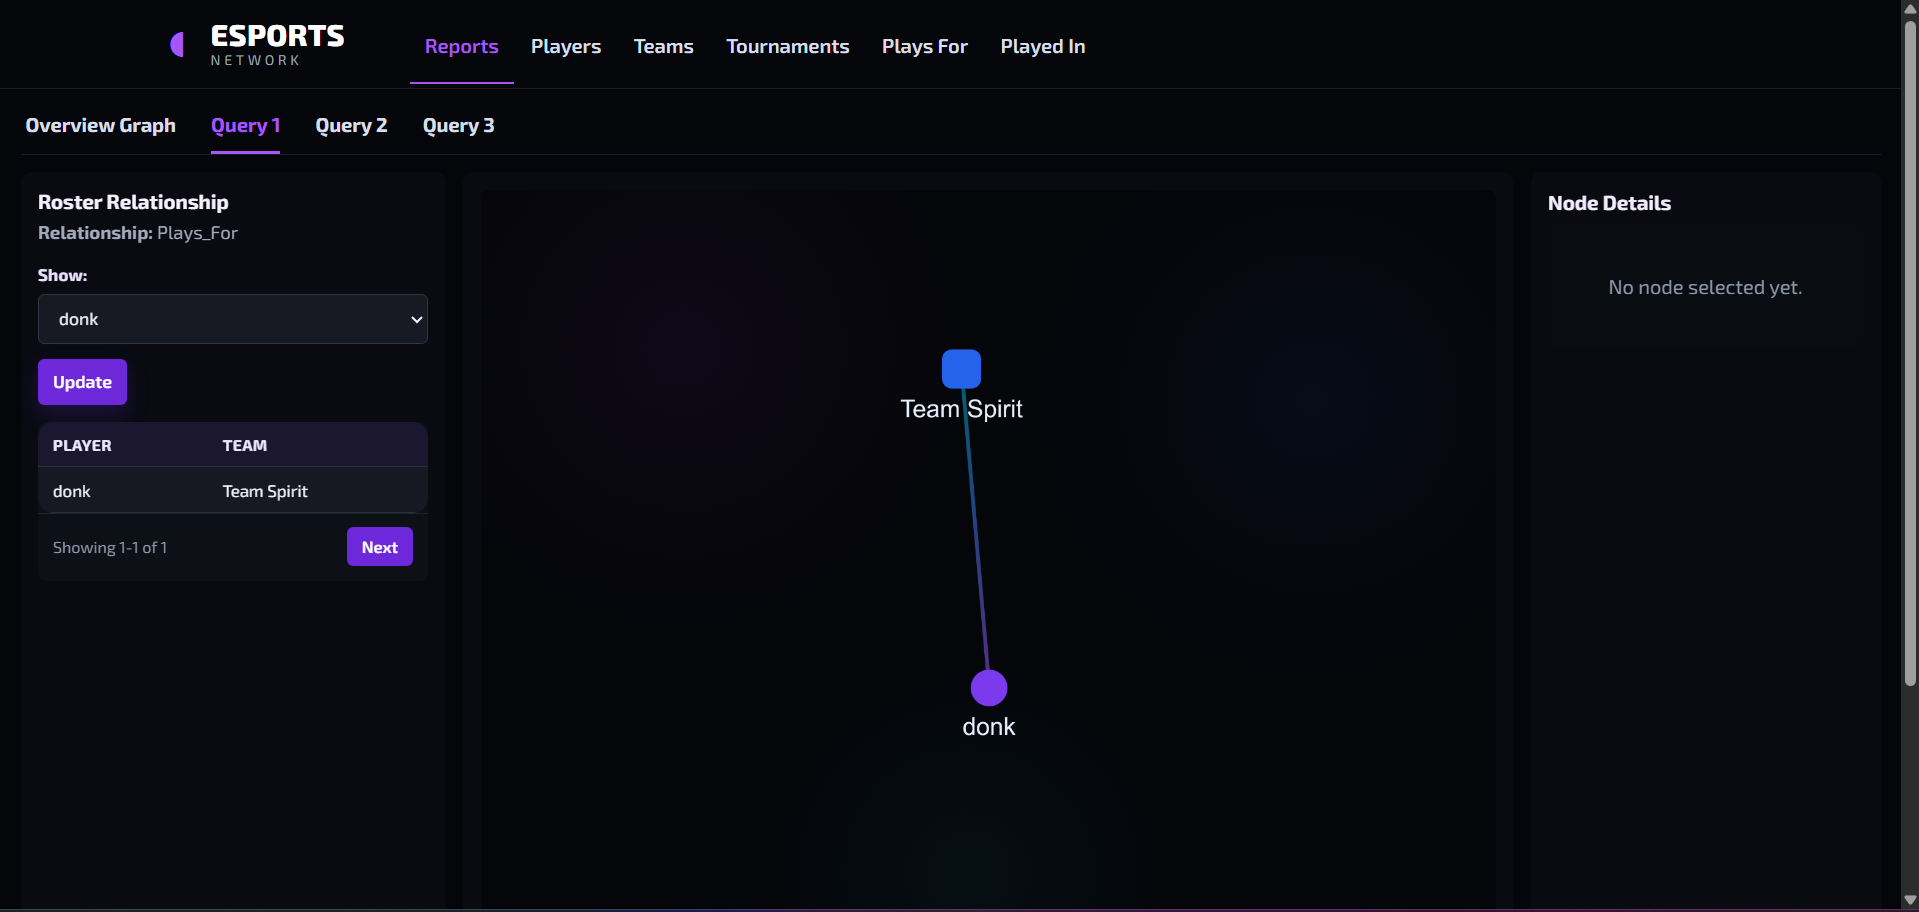
\includegraphics[width=1\linewidth]{images/ESports-Q1Example.png}
    \caption{Query 1 Webpage with Example}
    \label{fig:placeholder}
\end{figure}
\subsection{Query 2}
For this project the initial guidelines were to implement a \textit{h-index filer}. Which we implemented as a team filter based on both number of tournaments participated in and number won. Which takes a specific a specific number to represent the h-index. Then applies a filter on the teams and then presents that graphically with the tournaments and teams that participated in them. The first two queries are executed then the following two are applied to filter based on wins or particpation respectivly. Figure 6 showcases the webpage itself.
\begin{verbatim}
SELECT SourceNodeID, COUNT(DISTINCT TargetNodeID) 
    AS participant_count
    FROM Edges
    WHERE EdgeType = "Played_In"
    GROUP BY SourceNodeID  
SELECT NodeID, Name, NodeType, Attributes
    FROM Nodes
    WHERE NodeType = "Team"
    ORDER BY Name
    
SELECT e.EdgeID, e.SourceNodeID, e.TargetNodeID,
    tr.Name AS tournament_name, 
    tr.Attributes AS tournament_attributes
    FROM Edges e
    JOIN Nodes tr ON tr.NodeID = e.SourceNodeID
    WHERE e.EdgeType = "Won_By"
      AND tr.NodeType = "Tournament"
    ORDER BY tr.Name




SELECT e.EdgeID, e.SourceNodeID, e.TargetNodeID,
    tr.Name AS tournament_name, 
    tr.Attributes AS tournament_attributes
    FROM Edges e
    JOIN Nodes tr ON tr.NodeID = e.SourceNodeID
    WHERE e.EdgeType = "Played_In"
      AND tr.NodeType = "Tournament"
    ORDER BY tr.Name
\end{verbatim}
\begin{figure}[H]
    \centering
    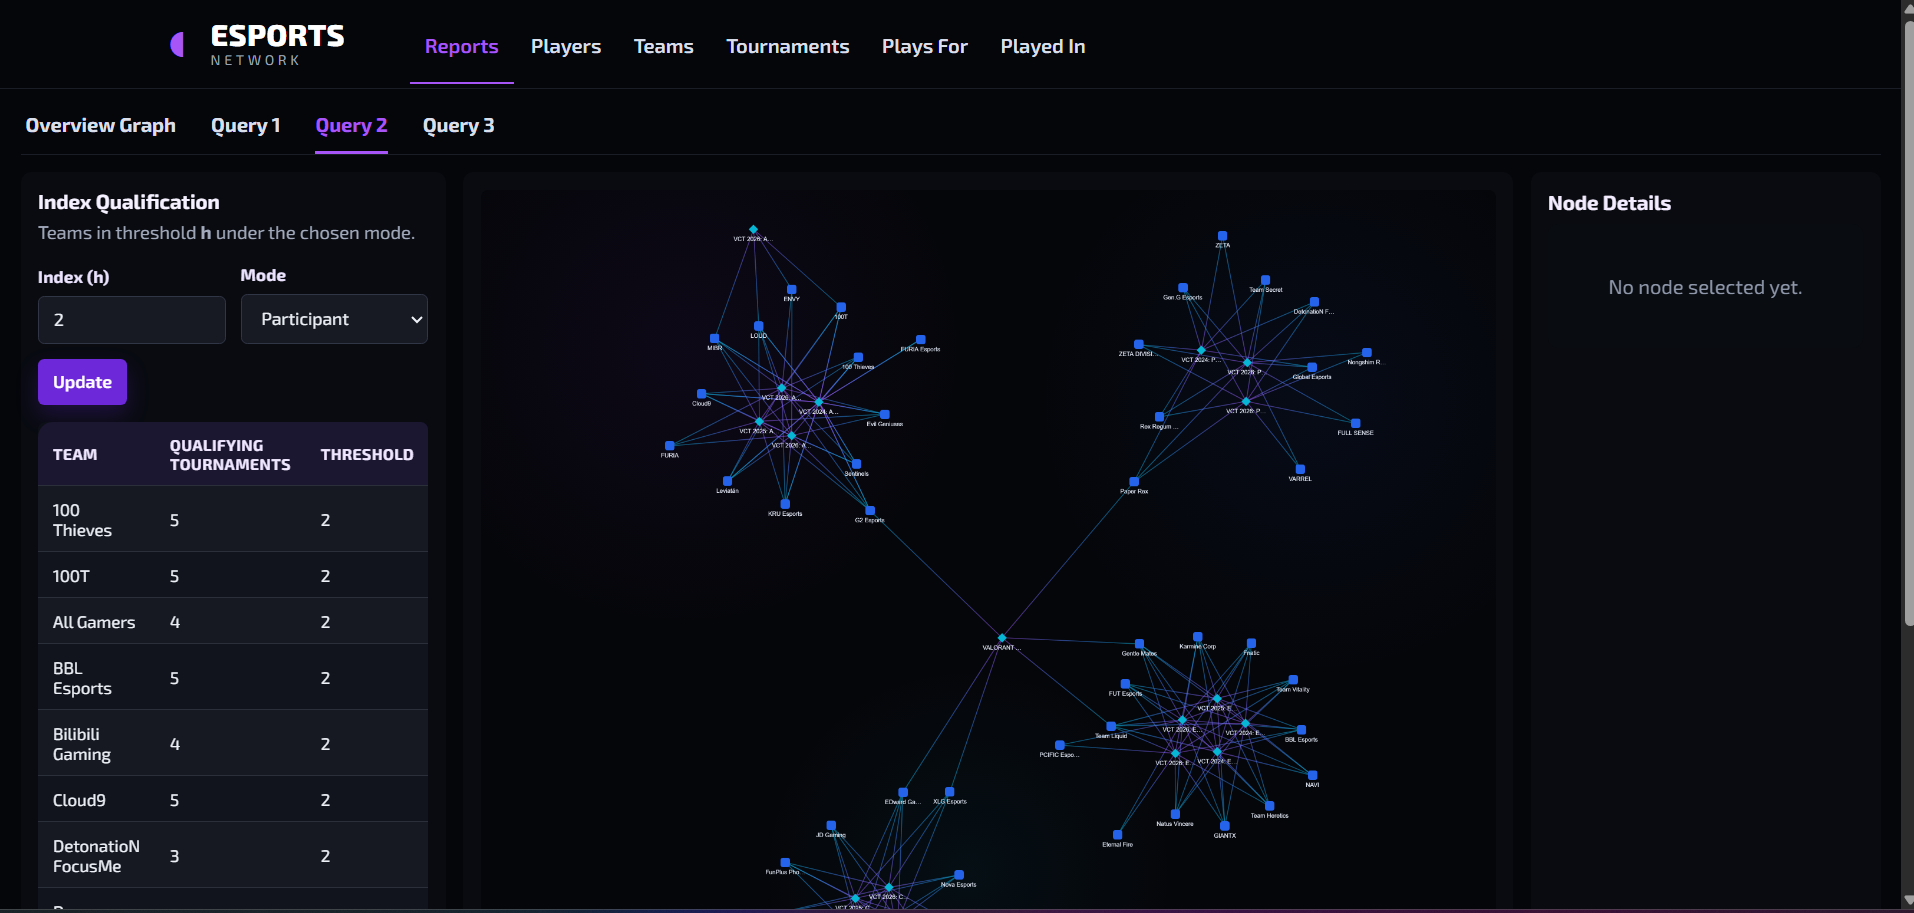
\includegraphics[width=1\linewidth]{images/ESports-Q2.png}
    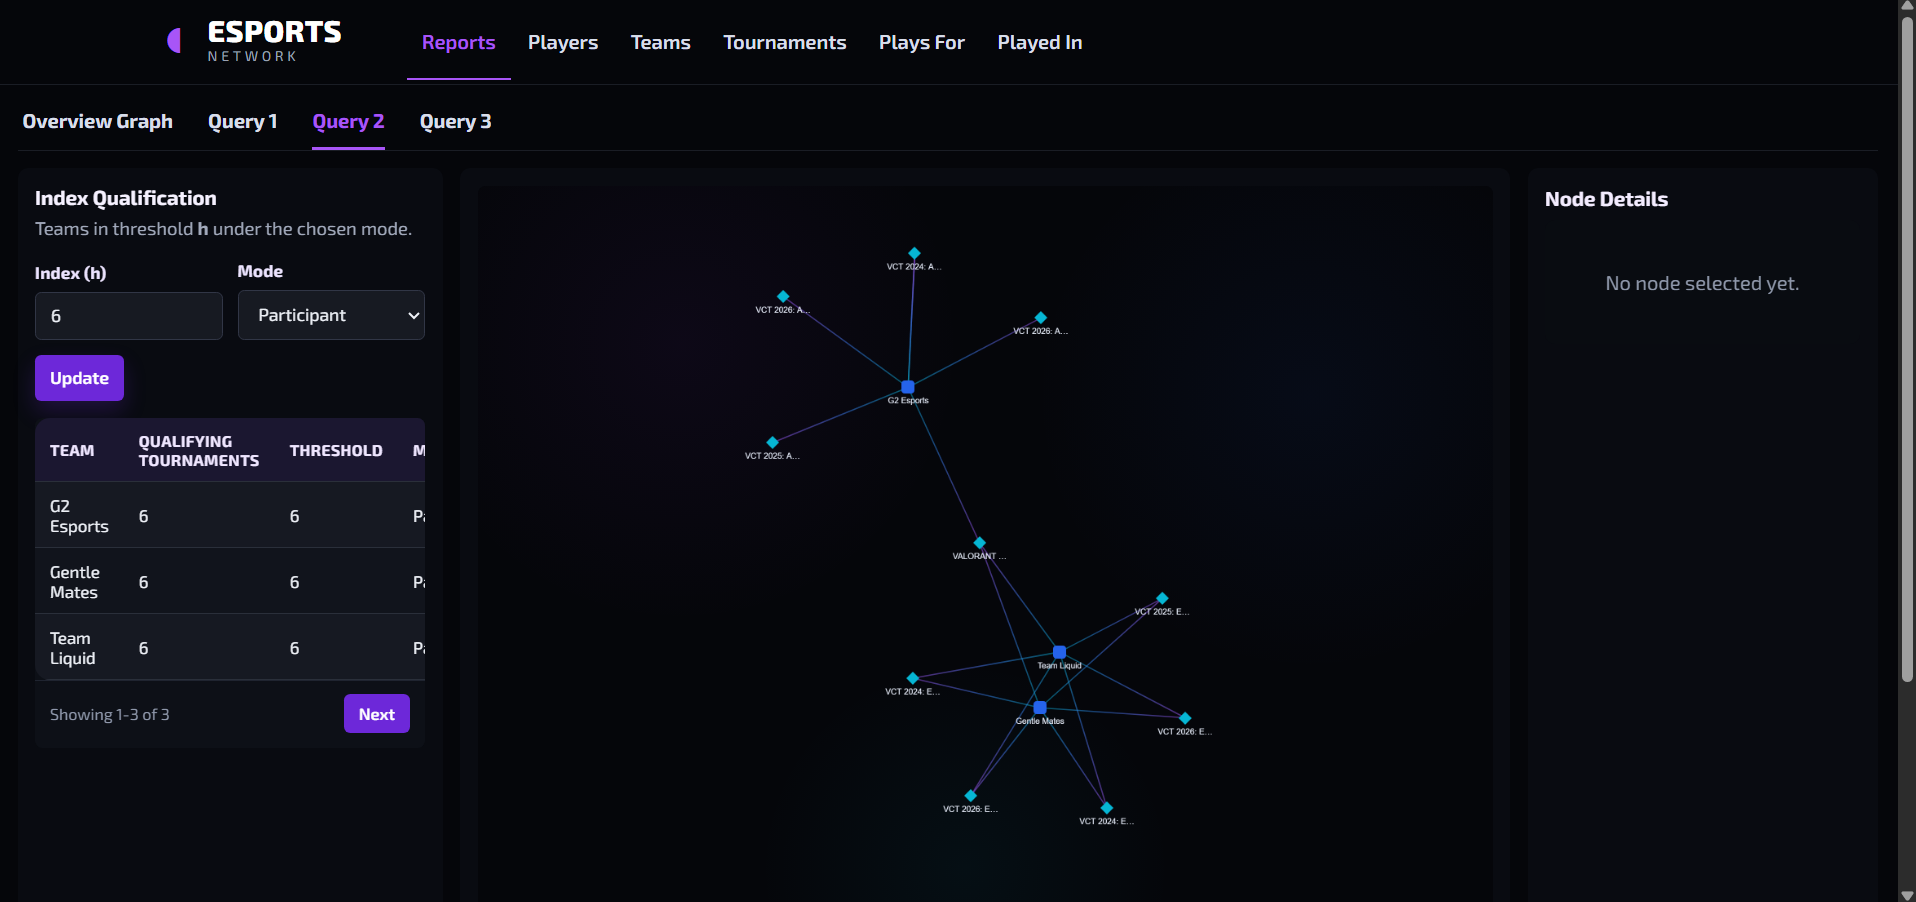
\includegraphics[width=1\linewidth]{images/ESports-Q2Example1.png}
    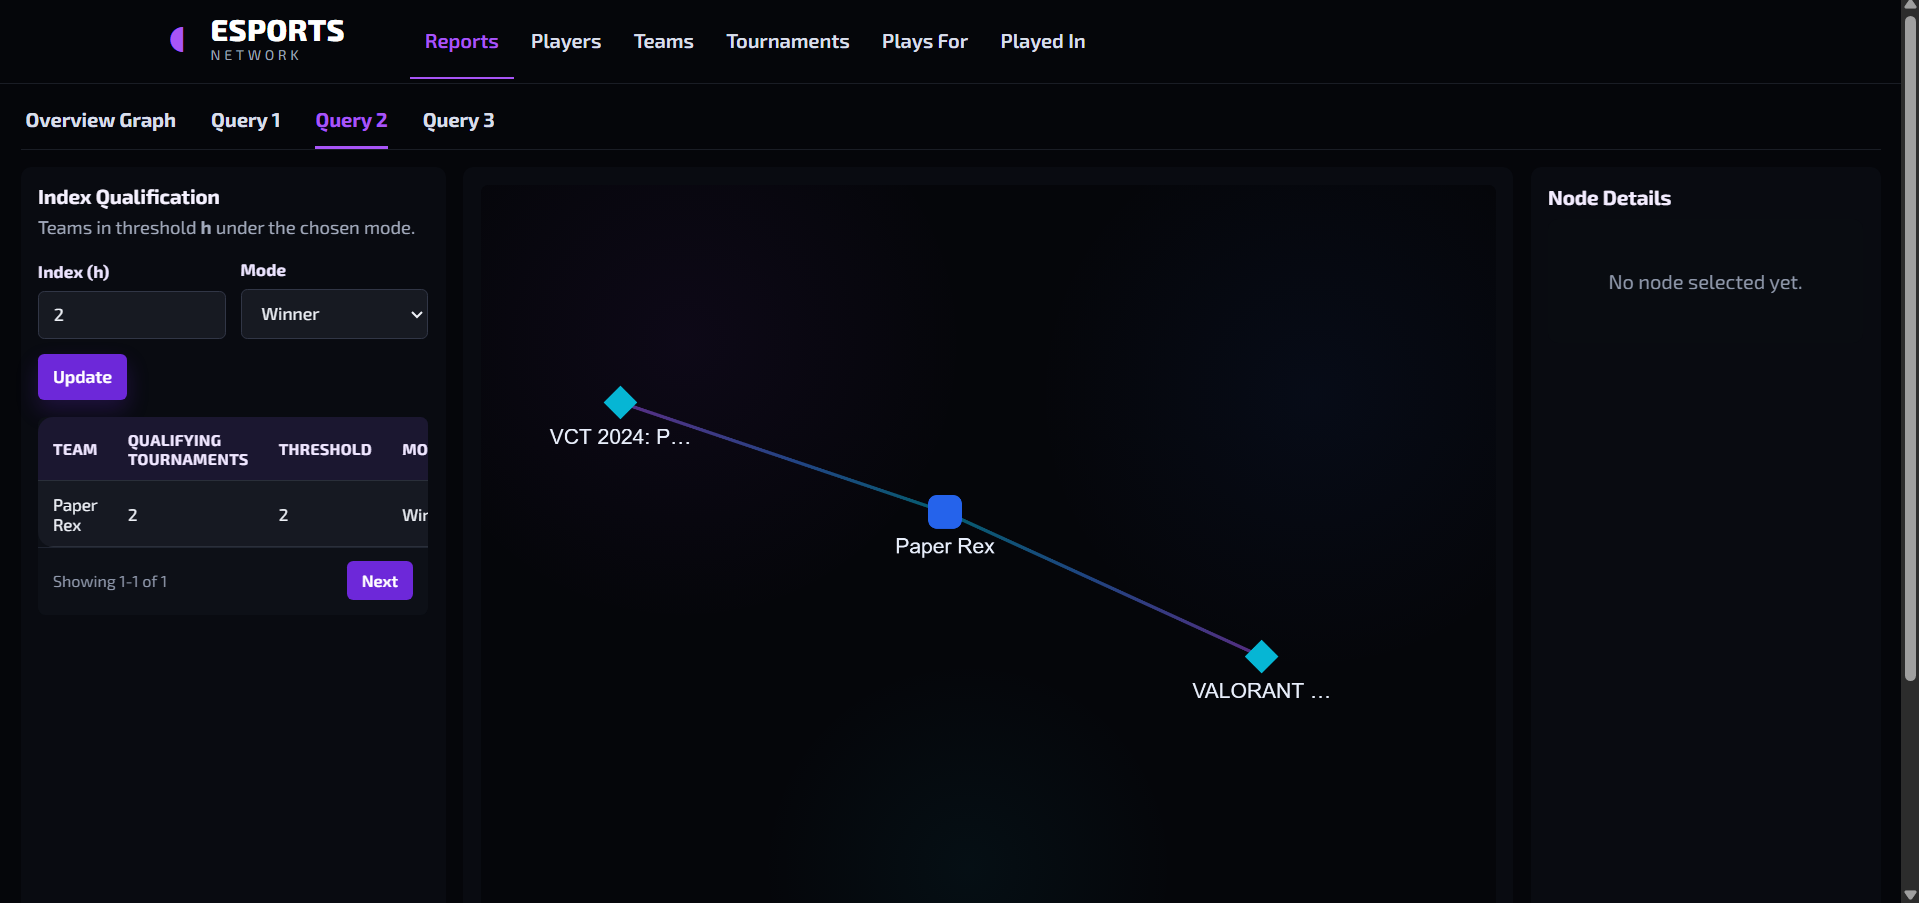
\includegraphics[width=1\linewidth]{images/ESports-Q2Example2.png}
    \caption{Query 2 Webpage with Examples}
    \label{fig:placeholder}
\end{figure}
\subsection{Query 3}
For this project the guidelines were to implement a \textit{Q1 Journal Influence Network}. Which we implemented as a Q1 Tournaments filter. We defined a Q1 tournament as a tournament where the prize pool is greater than 1 million dollars. The influence network of a Q1 tournament is all teams that participated in that tournament. For this query the below statements are executed, first getting the qualifying tournaments, then all teams that are associated with it and all matching edges. Figure 7 showcases the webpage.

\begin{verbatim}



SELECT DISTINCT n.NodeID, n.Name, n.NodeType, n.Attributes
    FROM Nodes n
    JOIN GraphMemberships gm ON gm.NodeID = n.NodeID
    WHERE gm.GraphID = 3
    AND n.NodeType = "Tournament"
    ORDER BY n.Name

SELECT DISTINCT n.NodeID, n.Name, n.NodeType, n.Attributes
    FROM Nodes n
    JOIN GraphMemberships gm ON gm.NodeID = n.NodeID
    WHERE gm.GraphID = 3
    AND n.NodeType = "Team"
    ORDER BY n.Name

SELECT DISTINCT e.EdgeID, e.SourceNodeID, e.TargetNodeID, 
    e.EdgeType
    FROM Edges e
    JOIN GraphMemberships gm ON gm.EdgeID = e.EdgeID
    WHERE gm.GraphID = 3
    AND e.EdgeType IN ("Played_In", "Won_By")
    ORDER BY e.EdgeID
\end{verbatim}

\begin{figure}[H]
    \centering
    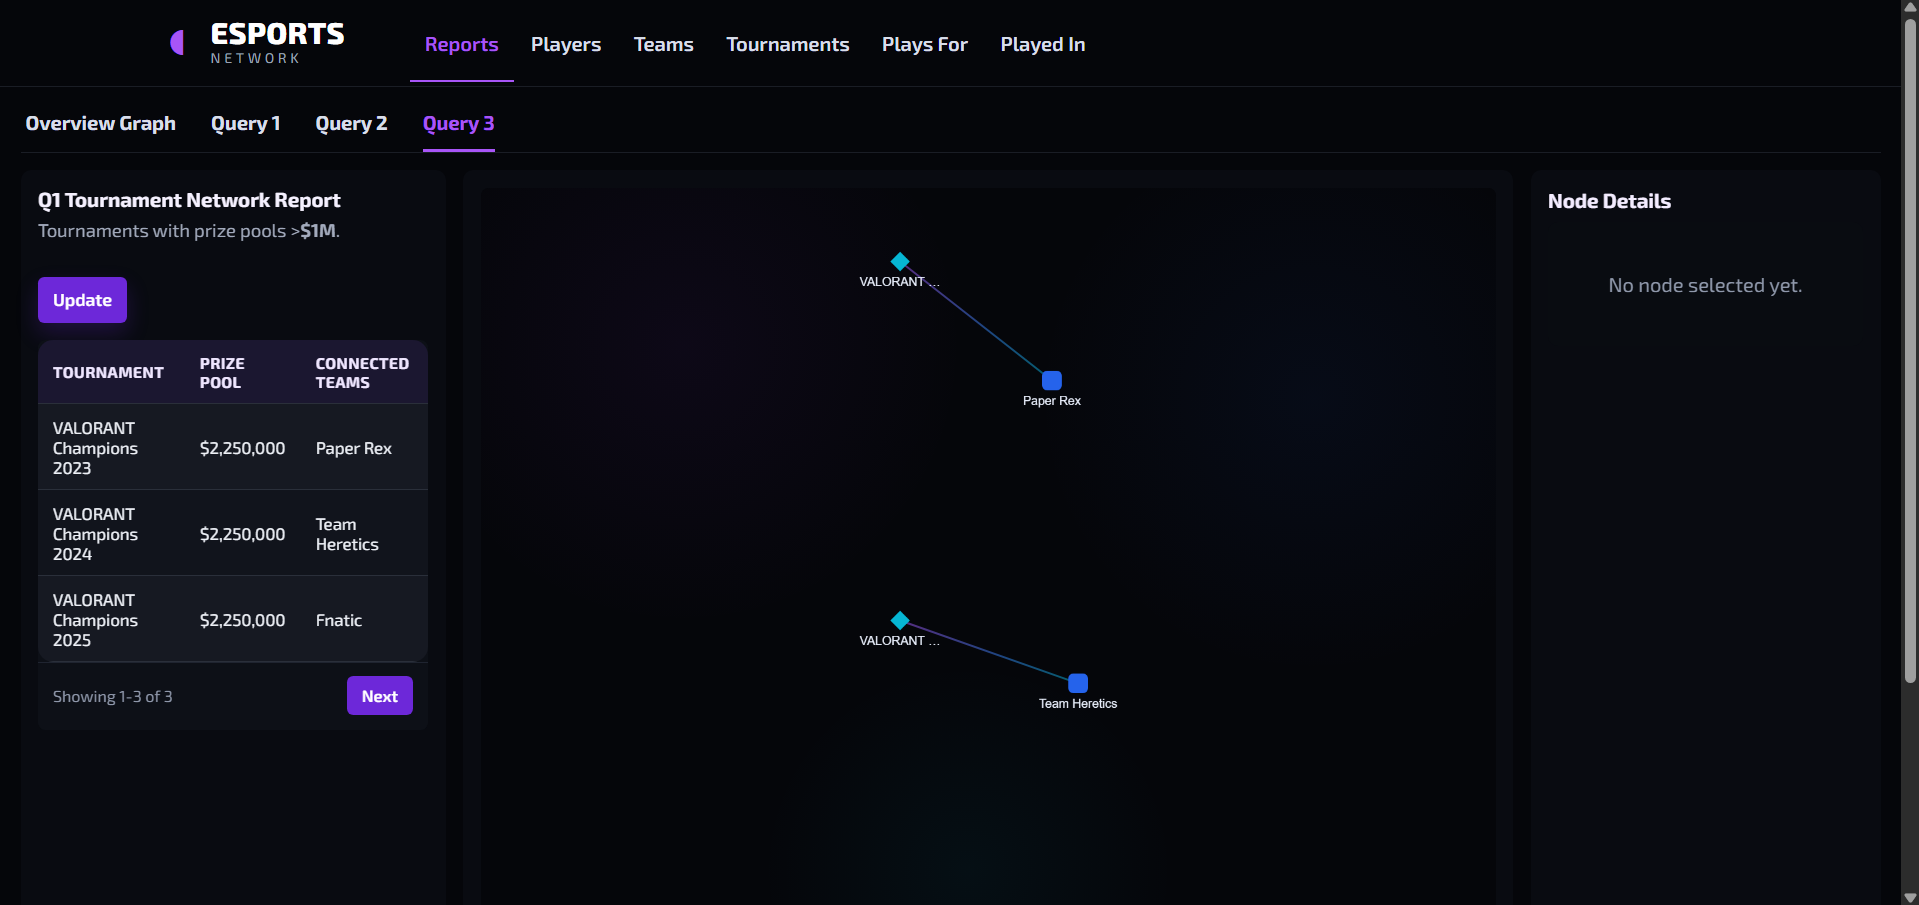
\includegraphics[width=1\linewidth]{images/ESports-Q3.png}
    \caption{Query 3 Webpage with Example}
    \label{fig:placeholder}
\end{figure}

\subsection{Timeline Comparison}
Below is the timeline outlined in phase one.
\begin{itemize}
    \item Phase 1: 
    \begin{itemize}
        \item Initial Design Presentation\\Date: March 3rd
        \item Initial Project Outline Report\\Date: March 7th
    \end{itemize}
    \item Phase 2: 
    \begin{itemize}
        \item Working Prototype Presentation\\Date: March 24th
        \item General Design Report\\Date: March 28th
    \end{itemize}
    \item Phase 3:
    \begin{itemize}
        \item Fully Function Prototype Presentation\\Date: April 21st
        \item Expanded Design Report\\Date: April 25th
    \end{itemize}
    \item Phase 4:
    \begin{itemize}
        \item Final Project Demo\\Date: May 5th
        \item Finalized Project Report\\Date: May 3rd
    \end{itemize}
\end{itemize}
As of writing this report it's clear we are on track to complete phase four on time. The initial project has been outlined and created. The initial prototype was created allowing for population of the database. As well as initial database schema was defined and them later revised. The functional prototype has been demonstrated in this report. As well as the three required queries co-author network, h-index filter, and Q1-journal influence network.
\section{Conclusion}
E-Sports has rapidly evolved into a global form of entertainment across titles such as \textit{League of Legends}, \textit{Counter-Strike}, and \textit{Dota 2}. Despite this growth, the analytical infrastructure supporting e-sports still lags behind traditional sports. The E-Sports Competitive Network directly addresses this limitation by introducing a relational database designed to model the relationships between players, teams, and tournaments across multiple games. These relationships are showcased through an updated relationship schema and tech stack. The E-Sports Competitive Network allows for mass population of it's database through a custom developed web scrapper and manual insertion through its web pages. The E-Sports Competitive Network features three key queries, the teammate network which showcases how players are related across teams. A h-index filter to showcase teams based on the number or tournaments they've participated in as well as won. Lastly, the Q1 journal influence network which showcases all teams that have participated in a tournament with a prize pool over 1 million dollars. The E-Sports Competitive Network lays the groundwork for more advanced analytical tools that can benefit coaches, analysts, and researchers.
\bibliographystyle{ACM-Reference-Format}
\bibliography{references.bib}
\cite{Shannon2003Cytoscape}
\cite{playwright_python}

\end{document}
\endinput
%%
%% End of file `main.tex'.
